\section{Contexte}
En l'état actuel, lorsque les pompiers doivent intervenir dans le cas d'un incident impliquant des fuites d'hydrocarbures sur route, la répartition
du produit absorbant se fait via une remorque-semoirs dont les sections de dépose du produit sont télécommandées directement par un opérateur.
Cela signifie que durant l'intervention, une personne doit marcher à côté de la remorque afin d'observer et contrôler la répartition du produit, nous pouvons relever les problèmes suivant:
\begin{enumerate}
    \item L'opérateur doit marcher: Limitation de la vitesse du véhicule, longues distances épuisantes.
    \item La détection se fait à l'oeil nu: L'opérateur doit rester concentrer en permanance au risque de devoir repasser sur certaines zone.
    \item La commande est manuelle: Possibilité d'erreur humaine sur la commande risquant la dépose de surplus de produit ou de devoir repasser sur certaines zone.
\end{enumerate}
\textbf{Le but de se travail de Bachelor est d'automatiser ce processus, via un système de détection des hydrocarbures par vision industrielle et d'un pilotage des vérins électronique.}
\section{Cahier des charges \label{cdc}}
Le cahier des charges se présente sous la forme suivante:
\begin{itemize}
    \item \textbf{Système de vsion pour détecter les hydrocarbures.}
          \begin{itemize}
              \item Sélectionner et mettre en place un éclairage adapté.
              \item Sélectionner et mettre en place un capteur adapté à l'éclairage.
              \item Définir un boitier de traitement.
          \end{itemize}
    \item \textbf{Commande des vérins du semoir.}
          \begin{itemize}
              \item Conceptualiser et mettre en place un système non-intrusif pour piloter les vérins du semoir.
          \end{itemize}
    \item \textbf{Retour vidéo pour le pilote de la voiture.}
          \begin{itemize}
              \item Sélectionner et mettre en place une méthode de retour vidéo permettant au pilote/co-pilote d'avoir un aperçu de la situation au niveau du semoir.
          \end{itemize}
\end{itemize}
\section{Planning}
Le planning vient compléter le cahier des charges du chapitre \ref{cdc} en ajoutant le travail à effectuer pour chaque étape ainsi qu'une estimation
de l'effort à fournir en heure.

Le planning ci-dessous présente les étapes, le détail des sous-étapes, l'effort à fournir estimé ainsi que la période dans laquelle chaque étape seront présumément effectuée (en bleu).
\begin{figure}[H]
    \centering
    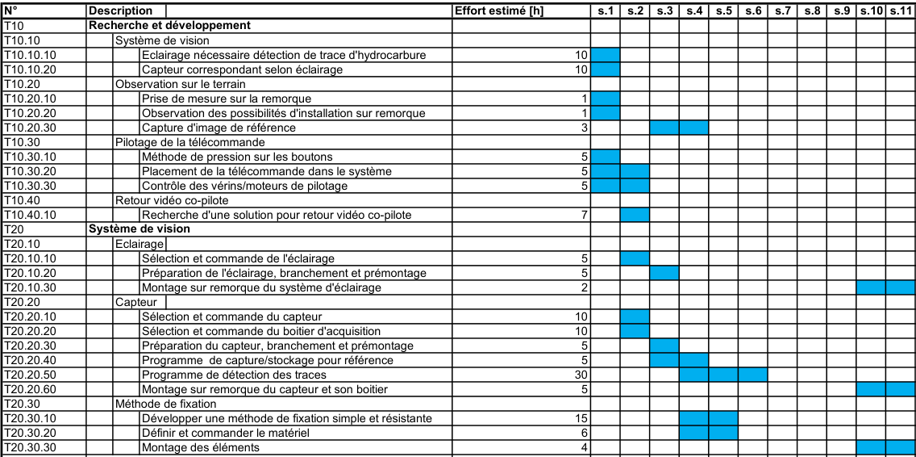
\includegraphics[width=15cm, angle=90]{assets/figures/planning1.png}
    \caption{Planning - partie 1}
\end{figure}
\newpage
\begin{figure}[H]
    \centering
    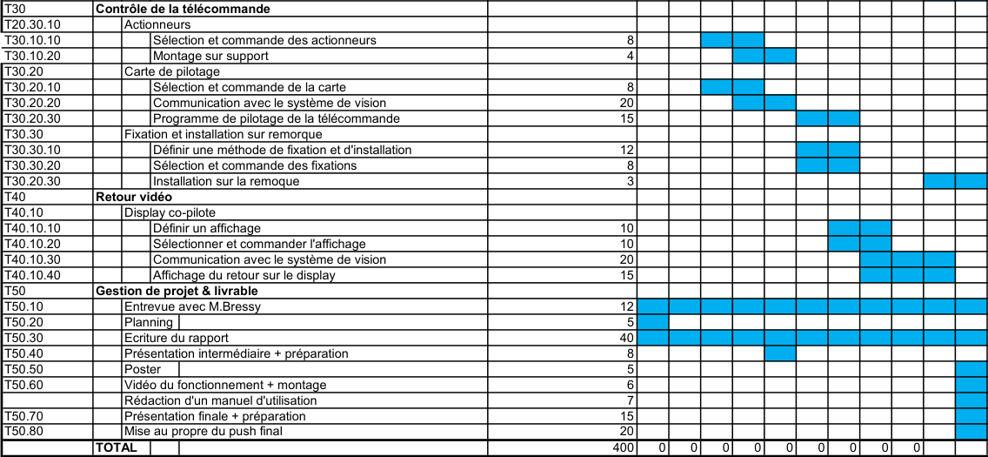
\includegraphics[width=15cm, angle=90]{assets/figures/planning2.png}
    \caption{Planning - partie 2}
\end{figure}

En complément au planning ci-dessus, on peut imaginer une vingtaine d'heures d'imprévus supplémentaires.
\iffalse
    %%if
    \section{Citations et bibliographie}
    Citer vos sources est essentiel. Avec \texttt{biblatex} vous pouvez facilement citer des articles, des livres ou des sites internet. Toutes les citations dans le texte seront automatiquement regroupées en fin de document dans la section \guillemotleft Bibliographie\guillemotright. Par exemple, citons un article d'Einstein \cite{einstein} ou le livre de Dirac \cite{dirac}.
    
    Parfois il peut être utile d'utiliser un gestionnaire de bibliographie. La communauté académique recommande l'outil \href{https://www.zotero.org/}{Zotero} qui permet de gérer une bibliothèque numérique d'ouvrages et de références numériques. Il permet également de générer une bibliographie compatible avec \LaTeX.
    
    Notez qu'il est très facile d'obtenir l'extrait \texttt{bibtex} depuis des journaux. Sélectionnez \emph{export/citation}. Si vous le pouvez choisissez \texttt{bibtex}. Dans le cas d'un format \texttt{.ris}, utilisez un convertisseur en ligne comme \href{http://www.bruot.org/ris2bib/}{ris2bib}.
    
    \section{Adapter votre modèle}
    Ce document n'est qu'un modèle ayant pour but de revoir les quelques avantages de \LaTeX~ et les fonctionnalités qui pourraient vous être utiles pour rédiger un rapport académique. N'hésitez pas à supprimer les parties inutiles et à adapter ce modèle à vos besoins.
    %%fi
\fi